\section{RANSAC}
\subsection{Motivation}
In einem der in dieser Arbeit vorgestellten Ansätze zur Fahrspurverfolgung soll ein Modell, genauer ein Polynom 3. Grades, gefunden werden, welches den Verlauf einer Fahrbahnmarkierung möglichst exakt darstellt. Nachdem auf den Bilddaten eine Kantenextraktion ausgeführt wurde, stehen nun mögliche Kandidaten für Punkte der Fahrspurmarkierung fest. Durch ungünstige Beleuchtungsverhältnisse, verschmutzte Fahrbahnen oder andere Störeinflüsse enthalten diese Punktmengen oft Ausreißer, welche bei einer Regression durch die Methode der kleinsten Fehlerquadrate für falsche Modelle sorgen würden. \gls{acr:ransac} \autocite{fischler1981random} ist ein Algorithmus um solche Ausreißer zu entfernen.

\begin{figure}[H]
  \centering
  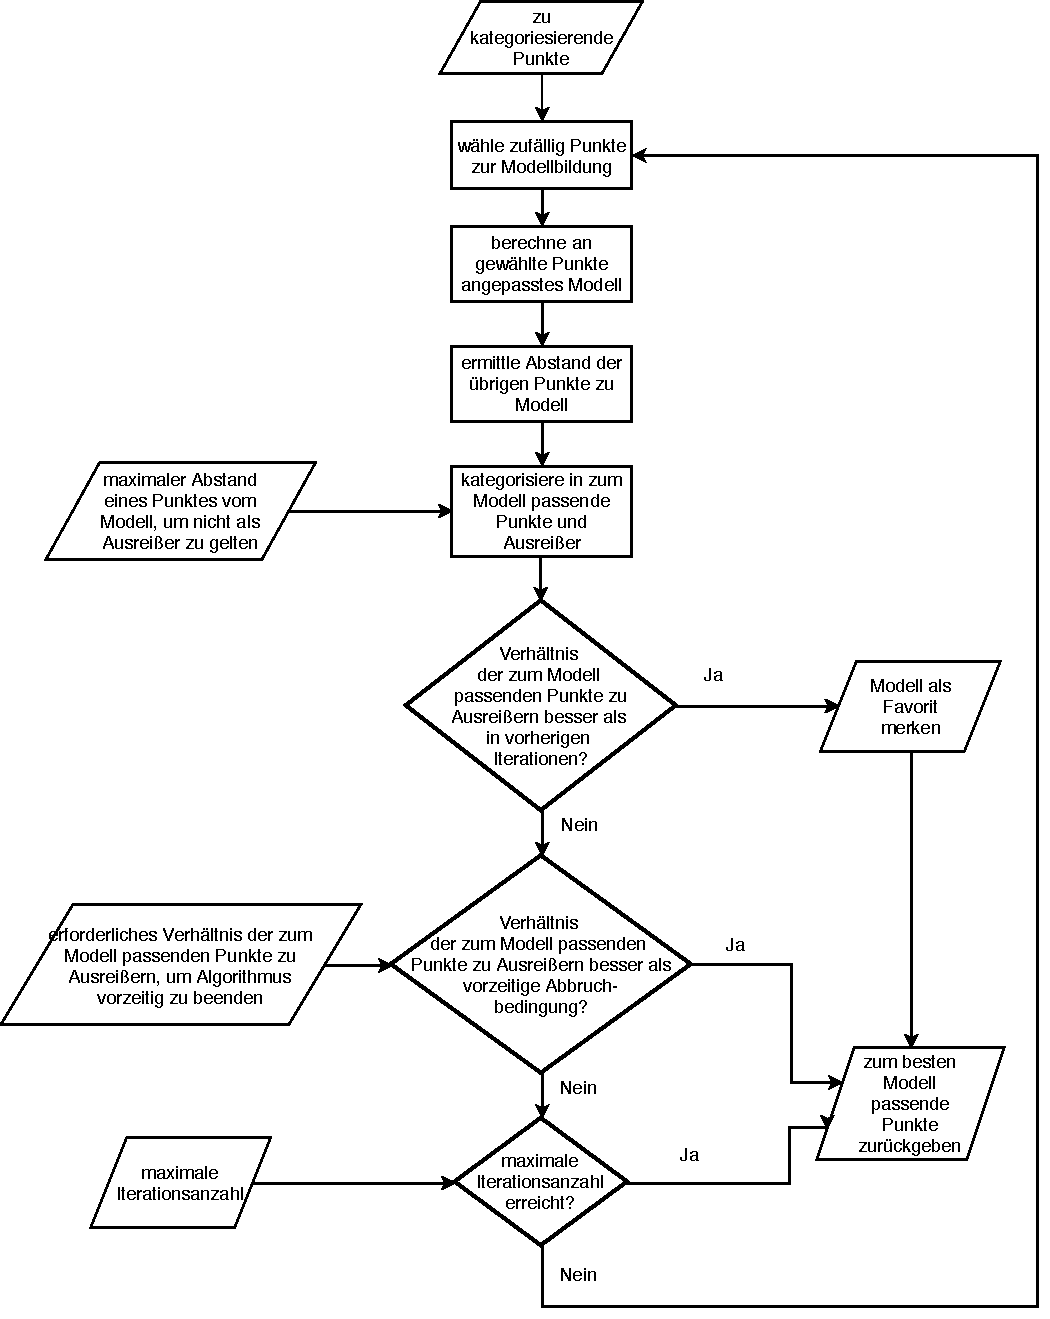
\includegraphics[width=1\textwidth]{Ransac_Schema}
  \caption{Schema zum Ablauf des \gls{acr:ransac}-Algorithmus}
  \label{fig:ransac_scheme}
\end{figure}

\subsection{Ablauf des Algorithmus}
In jeder Iteration wählt der Algorithmus zufällig mindestens so viele Punkte aus dem ihm übergebenen Datensatz, wie für die Bildung des Modells notwendig sind. Das Modell auf Basis dieser Punkte wird nun errechnet. Den nächsten Schritt stellt die Ermittlung des Abstandes der übrigen Punkte des Datensatzes vom gefundenen Modell dar. Punkte mit einem Abstand kleiner als ein festgelegter Schwellwert zählen als sogenannte \gls{glos:inlier}. Ist das Verhältnis der Anzahl von \glspl{glos:inlier} zu \glspl{glos:outlier} besser als in allen vorherigen Iterationen, wird das Modell vorgemerkt. Ist das Verhältnis von \glspl{glos:inlier} zu \glspl{glos:outlier} sogar besser als ein festgelegter Schwellwert, bricht der Algorithmus vor dem Erreichen einer maximalen Iterationsanzahl ab, andernfalls wird er bis zum Erreichen selbiger wiederholt.

\subsection{Nachfolgende Schritte}
Das gefundene Modell mit den dazugehörigen, als \gls{glos:inlier} gefundenen Punkten kann nun mit der Methode der kleinsten Quadrate weiter optimiert werden.




